\documentclass[]{vgtuef}
\usepackage[utf8x]{inputenc}
\usepackage[L7x]{fontenc}
\usepackage[lithuanian]{babel}

\author{Tomas Fedosejev, Marius Buinevičius\\Vilniaus Gedimino technikos
  universitetas\\Elektronikos fakultetas\\Elektroninių sistemų
  katedra\\\texttt{tomas@fedosejev.lt}}
\title{Bakalauro baigiamasis darbas\\Virtualios garso realybės sistema}


\begin{document}

\setcounter{page}{7}

\onehalfspacing

\tableofcontents


\section*{Žymenys ir santrumpos}
\addcontentsline{toc}{section}{Žymenys ir santrumpos}

\begin{itemize}
\item HRTF - su galva susijusios perdavimo funkcijos (angl. \textit{Head Related Transfer Function}).
\item ATF - anatominė perdavimo funkcija (angl. \textit{Anatomical Transfer Function}).
\item FFTF - (angl. \textit{Field-Free Transfer Function}).
\item RIR - kambario impulsinis atsakas (angl. \textit{Room Impulse Response}).
\item HRIR - (angl. \textit{Head Related Impulse Response}).
\item ITD - tarpausinis laiko skirtumas (angl. \textit{Interaural Time Difference}).
\item ILD - tarpausinis garso lygių skirtumas (angl. \textit{Initial Level Difference}).
\item USB - universalioji nuoseklioji jungtis (angl. \textit{Universal Serial Bus}).
\item COM - RS232 nuoseklusis prievadas.

\end{itemize}


\section{Įvadas. Užduoties analizė}

Darbo tema yra "Virtualios garso realybės sistema". Šiuo metu virtualio ir papildytos realybės programinė įranga yra toli pažengusi, tačiau garso generacijai taip ir toliau naudojamas stereo garsas, kuriuo nėra įmanoma tiksliai atkurti aplinkos garsus.
Šiuo darbu siekiama ištirti galimybes sukurti realiuoju laiku veikiančia sistemą gebančią generuoti binauralinį garsą priklausomai nuo vartotojo galvos orientacijos ir virtualios aplinkos akustinių parametrų. Sistema yra suskirtyta į tris pagrindines dalis: galvos sekimo įrenginį - kuris seka vartotojo galvos orientaciją; programą asmeniniame kompiuteryje - kuri siunčia virtualios aplinkos duomenis ir garso šaltinio skleidžiamą garsą; garso apdorojimo įrenginį - kuris apjungia informaciją gautą iš galvos sekimo įrenginio bei asmeninio kompiuterio ir sugeneruoja binauralinį garsą. Tokia architektūra buvo pasirinka dėl modulinės struktūros, be to perkėlus garso generavimą į atskirą įrenginį, atlaisvinamas asmeninio kompiuterio centrinis procesorius, ko pasekoje virtualiai aplinkai sukurti lieka daugiau asmeninio kompiuterio resursų.
Pradiniai bandymai bus atlikti \textit{Matlab} terpėje, kas leis įsitikinti sistemos įgyvendinimo galimybėmis, bei duos progą patobulinti naudojamus procesus.
Virtualios garso realybės tema buvo pasirinkta dėl savo prespektyvumo, nors binauralinis garsas pradėtas tirti pakankamai seniai, realiai veikiančių įrenginių nėra sukurta. Tema yra aktuali žaidimų ir medicinos pramonei.
Didžiausia sistemos problema slypi HRTF (angl. \textit{Head Related Transfer Functions}) panaudojime, kadangi HRTF deriniai turi būti pritaikyti individualiai kiekvienam klausytojui. Tačiau panaudojus papildomus procesus garso generavimo eigoje, pamėginta sumažinti HRTF neigiamą įtaką.
Darbo eigoje bus sukurta pilnai veikianti sistema gebanti kuo tiksliau atkurti virtualią akustinę aplinką, programinė įranga bus parašyta garso apdorojimo, galvos orientacijos įrenginiams, bei asmeniniam kompiuteriui. Taip pat bus suprojektuoti abu naudojami įrenginiai.
Baigiamojo bakalaurinio darbo sistemos asmeninio kompiuterio programinei įrangai reikalingi mažiausiai 20MB diskinio kaupiklio dalies talpos. Toks atminties kiekis reikalingas norint vartotojo sąsają padaryti patrauklesnę vartotojui, t.y. grafinės iliustracijos, garsai ir kt. Asmeniniame kompiuteryje programinė įranga dirba Windows 7 operacinėje sistemoje, nes senesnių operacinių sistemų versijų (XP, Vista) Microsoft korporacijos palaikymas bus nutraukiamas artimiausiu metu.
Garso apdorojimo įrenginyje bus naudojama ne mažesnė nei 1.1 USB lizdo versija, nes sistema suprojektuota darbui su šia ar aukštesnėmis versijomis. Duomenų perdavimą taipogi būtų galima realizuoti ir kitomis sąsajomis, tokiomis kaip COM, bet tokiu atveju greitis būtų nepakankamas ir sistema įgautų netoleruotiną vėlinimą. Be to, binauralinio garso generavimo sistema yra šiuolaikinė ir labiau taikintina nešiojamiems kompiuteriams, kuriuose nebediegiami RS232 prievadai. Išlieka galimybė naudoti RS232 prievadą, bet tokiu atveju tektų papildomai turėti iš USB į COM keitiklio kabelį, kuris taip pat naudoja USB jungtį. Todėl geriausias pasirinkimas spartos atžvilgiu rinktis virtualų COM  prievadą per USB jungtį.
Siekiant išlaikyti kuriamos sistemos kuo ilgesnį autonominio veikimo laiką sistema toleruoja maksimalų 0,5 A srovės suvartojimą (tiek galvos orientacijos nustatymo įrenginys tiek garso apdorojimo įrenginys), be to 0,5 A tai didžiausia srovė kurią pagal specifikaciją gali atiduoti USB 1.1 ir USB 2.0 prievadai.
Norint išlaikyti sistemos mobilumą, kurio didžioji dalis priklauso nuo galvos sekimo įrenginio dydžio, buvo pasirinkti pakankamai nedideli pastarojo įrenginio maksimalūs matmenys: 50 × 100 × 100 mm.  
Sistemos veikimas bus vertinamas sugeneruoto binauralinio garso tikslumu (palyginus su įrašytu binauraliniu garsu), bei autonominio veikimo trukme.


\section{Analogiškų sistemų apžvalga}

Šiame skyriuje bus apžvelgtos analogiškos sistemos: buvę prototipai ir šiuo metu esami rinkoje produktai. Apibendrintai bus aptarti nagrinėjamų sistemų teigiamos ir neigiamos savybės. 


Galvos sekimo įrenginio kūrimas nėra naujiena. Tokie įrenginiai naudojami norint nusakyti lėktuvų  trimatę poziciją. Pati \textit{sensor fusion} technologija taip pat jau gana ilgai naudojama aviacijos srityje, norint kur kas tiksliau nusakyti poziciją.
Kalbant apie binauralinio garso generavimą realiu laiku, paieškos rezultatai stipriai sumažėja. Tokio tipo projektų pasaulyje yra tik du. Projekto tikslai – binauralinio garso generavimas realiu laiku. Vienas iš projektų naudojo \textit{„Texas instruments“} pagamintą plokštę - C6713 DSK kuri pavaizduota \ref{fig:C6713_dsk_board} pav.

\begin{figure}[!ht]
  \centering
  \includegraphics[width=400px]{img/c6713.jpg}
  \caption{C6713 DSK spausdintinė plokštė.}
  \label{fig:C6713_dsk_board}
\end{figure}

Šios plokštės mikrovaldiklis dirba 225 MHz dažniu ir pasiekiantis 1800 milijonų instrukcijų per sekundę spartą. Taip pat ši plokštė gali apdoroti aukštos kokybės 24 bitų skaitmeminį stereo garsą, turi 512 kB \textit{Flash} bei 16 MB \textit{SDRAM} atmintis. \textit{JTAG}\footnote{JTAG - Programavimo ir testavimo jungtis.} prieinamas per \textit{USB} jungtį.

Kaip teigia gaminio kūrėjai, jie generuoja binauralinį garsą naudojant specialų stereo filtrą suprogramuotą minėtoje plokštėje. Programinė įranga naudoja nuo galvos priklausančias impulso atsako funkcijas sugeneruotas \textit{„Floridos tarptautinio universiteto“} asmenų (nepaminėta kieno). Dviejų kanalų išėjimui panaudotos 12 \textit{HRTF} funkcijų, kurios taip pat nebuvo sugeneruotos projekto autorių. 

Kūrėjų teigimu, rezultatai jų stipriai nestebina – geriausias efektas jaučiamas tik garsui esant už galvos, nes panaudotos \textit{HRTF} funkcijos nėra pritaikytos jų ausims. Šio įrenginio testavimo akimirką demonstruoja \ref{fig:C6713_dsk_board_checkout} pav.

\begin{figure}[!ht]
  \centering
  \includegraphics[width=400px]{img/c6713_patikra.jpg}
  \caption{C6713 DSK plokštės patikra.}
  \label{fig:C6713_dsk_board_checkout}
\end{figure}


Kompiuterinis binauralinio garso generavimas yra įmanomas, bet reikalauja didelių kompiuterio resursų, taip atimdamas galią iš centrinio procesoriaus, todėl kuriamos išorinės garso plokštės, kurios nepriklausomai nuo kompiuterio procesoriaus gali generuoti binauralinį garsą naudojant \textit{HRTF} funkcijas.

Pirmoji garso rinkoje pasirodęs produktas galėjęs pasiūlyti trimatį pozicinį garso generavimą buvo 1998 išleista \textit{„Aureal Vortex via the A3D API“} garso plokštė. Deja nėra  galimybės jos išbandyti, bet pagal vartotojų atsiliepimus ši plokštė sugebėdavo gana gerai suformuoti trimačio garso pojūtį. Kadangi įmonė \textit{„Aureal“} pasitraukė iš rinkos, tai jos poziciją perėmė \textit{„Creative Inc.“} firma. Gerą garso kokybę bei neblogą trimačio garso efektą gali pasiūlyti tik labai brangios pastarosios įmonės garso plokštės – \textit{„X-Fi“}. 

Šiuo metu binauralinio garso generavimas realiu laiku priklausomas nuo vartotojo galvos pozicijos neturi jokių analogų. Kaip ir buvo minėta, atskirai abi dalys yra daugiau ar mažiau naudojamos pasaulinėje rinkoje, bet būtent šių dviejų sričių sujungimas yra visiškai unikalus, todėl analogiškų sistemų apžvalga čia yra neįmanoma.

Kaip buvo minėta apžvalgoje sistema pasiūlytame pavidale yra unikali ir perspektyvi. Šiuo metu rinkoje nėra įrenginių gebančių sugeneruoti bunauralinį garsą priklausomai nuo klausytojo galvos orientacijos. Rinkoje esantys analogai suteikia programuotojams galimybę įgyvendinti šį efektą naudojantis papildomais programiniais įrankiais, tačiau įrenginių gebančių tai padaryti savaime, be papildomo programuotojų įsikišimo - nėra.

\section{Naudojamų metodų apžvalga}

Šiame skyriuje bus apžvelgti metodai kuriais remiantis buvo sukurti matematiniai modeliai ir realios sistemos prototipas.

\subsection{HRTF funkcijos}

\textit{HRTF} (angl. \textit{Head Related Transfer Function}) dar vadinamos \textit{ATF} (angl. \textit{Anatomical Time Difference}) tai funkcijos nusakančios atsaką kurį kuris charakterizuoja, kaip žmogaus ausis priima garsą sklindantį iš tam tikro taško erdvėje. Panaudojus \textit{HRTF} porą, skirta kiekvienai ausiai, įmanoma sintezuoti binauralinį garsą taip sukuriant erdvės pojūtį.  
Žmogaus smegenys apskaičiuoja garso šaltinio poziciją erdvėje naudojantis: 1) garso užuominomis atkeliavusiomis į kiekvieną ausį (angl. \textit{monoaural cues}), 2) abiejų ausų garso užuominų palyginimu (angl. \textit{difference cues} arba \textit{binaural cues}). Pagrindinės garso užuominos yra:
\begin{enumerate}
\item Tarpausinis laiko skirtumas (angl. \textit{Interaural Time Difference})
\item Tarpausinis garso lygių skirtumas (angl. \textit{Interaural Level Difference})
\item Spektriniai skirtumai (angl. \textit{Spectral cues} arba \textit{Pinae effect})
\item Galvos šešėlis (angl. \textit{Head Shadow})
\item Pečių aidas (angl. \textit{Shoulder Echo})
\item Ankstyvieji atspindžiai (angl. \textit{Early Reflections})
\item Atgarsiai (angl. \textit{Reverberation})
\end{enumerate}

\textit{HRTF} aprašo tik dalį iš aukščiau pateiktų užuominų: TLS ir TGLS.


\subsection{Galvos šešėlis ir pečių aidas}

Galvos šešėlis arba dar kitaip vadinamas akustiniu šešėliu, tai sumažėjusios garso amplitudės regionas atsirandantis, nes galva sugeria arba sumažina amplitudę dalies ją pasiekusių garso bangų. Pasiekusi galvą garso banga gali keliauti aplink arba per galvą, kad pasiektų ausį esančią priešingoje pusėje. Tokiu būdu yra sukuriamas pakankamai geras pirminės lokalizacijos filtras. Ausį esančią šešėlyje garsas pasiekia maždaug 0,7 ms vėliau, ko pasekoje žmogaus smegenys sugeba nustatyti apytikslią garso sklidimo kryptį. 

Pečių aidas - tai aidas atsirandantis garso bangom atsispindėjus nuo klausytojo pečių. Toks aidas tiesiogiai turi mažai lokalizacijos informacijos tačiau sudėjus kartu su galvos šešėliu filtras dar labiau patikslėja.


\subsection{Tarpausinis laiko skirtumas}

TLS nusako laiko skirtumą tarp garso bangų pakliuvusių į dešiniąją ir kairiąją ausis, \ref{fig:ITD_1} paveikslas vizualiai parodo šio efekto veikimą. TLS – tai pirminė garso lokalizacijos užuomina padedanti nusakyti garso šaltinio padėtį erdvėje. Kadangi ausys yra atskirtos viena nuo kitos, garso banga nukeliauja skirtingą kelia prieš pasiekiant kiekvieną iš ausų.

\begin{figure}[!ht]
  \centering
  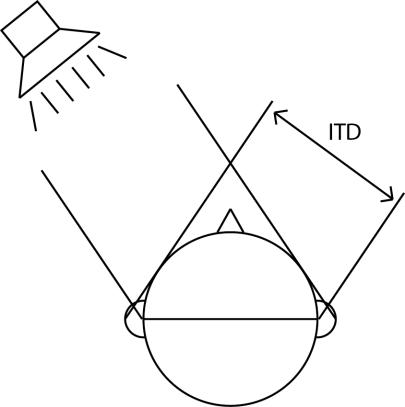
\includegraphics[width=150px]{img/ITD.jpg}
  \caption{TLS (angl. \textit{ITD}) efektas}
  \label{fig:ITD_1}
\end{figure}

Tačiau išimtį sudaro garsas esantis tiesiai prieš arba už klausytojo. TLS taip pat įtakoja garso bangos fazės  pakitimą. Jeigu fazių skirtumas didesnis nei 180 laipsnių, nustatyti kaip fazė yra pasislinkus tampa sunku. Žemuose dažniuose fazės skirtumas nusako pakankamai didelį laiko skirtumą ir yra naudingas orientacijos nustatymui. Aukšto dažnio signalams 180 laipsnių fazės poslinkis  nusakys mažesnį laiko skirtumą. Tai reiškia kad ši savybė tampa mažiau naudinga garso bangoms kurių dažnis priklausomai nuo kampo viršija 700-1500 Hz.

\subsection{Tarpausinis garso lygių skirtumas}
TGLS nusako garso stiprumo skirtumą tarp dviejų taškų (ausų). Šis reiškinys pasireiškia kai garso banga iš dalies yra blokuota galvos. Taip pat kaip ir TLS, TGLS negali tiksliai nusakyti skirtumo tarp garso esančio tiesiai prieš arba už klausytojo. TGLS efektas taipogi kaip ir TLS turi dažninę priklausomybę. Žemuose dažniuose dėl difrakcijos tik maža garso bangos dalis yra blokuota galvos, ko pasėkoje garso intensyvumo skirtumas pasidaro labai mažas.

Tačiau aukštų dažnių ruože difrakcija pasireiškia žymiai mažiau kas įtakoja žymiai didesni garso lygių skirtumą (\ref{fig:ILD_1} paveikslas). Kai kuriais atvejais garso lygių skirtumas gali sudaryti iki 20 dB. Todėl TGLS yra dažniausiai naudojamas aukšto dažnio garso bangoms, o TLS žemo dažnio bangų krypčiai nustatyti. 

\begin{figure}[!ht]
  \centering
  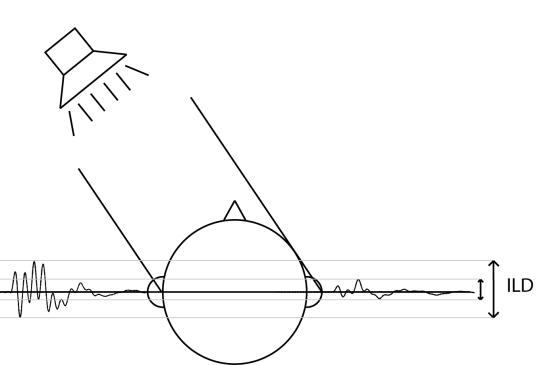
\includegraphics[width=150px]{img/ILD.jpg}
  \caption{TGLS (angl. \textit{ITD}) efektas}
  \label{fig:ILD_1}
\end{figure}

Taipogi labai svarbi yra spektrinė dedamoji (angl. \textit{pinnae effect}). Dėl kompleksinės ir asimetrinės ausies kriauklės formos garsas atsispindėjęs nuo ausies kriauklės spektriškai pasikeičia.  Kartu su pečių atspindžio efektu tai formuoja filtrą turintį krypties priklausomybę ir todėl ne taip kaip TLS ir TGLS yra įmanoma atskirti garsus sklindančius iš priekio ir iš galo. Dėl spektrinių pokyčių ši dedamoji geriausiai tinka atskirti plačiajuostį garsą - viršijantį 6 kHz dažnį.


\subsection{HRTF metodo panaudojimas}

Norint panaudoti šį metodą reikia turėti \textit{HRTF} rinkinį visiems vertikalių ir horizontalių kampų deriniams. Šiame darbe naudojami Masačiuseco technologijų instituto (angl. \textit{Massachusetts Institute of Technology}) 1994 metais atlikto projekto \textit{„KEMAR“} metu gauti universalūs \textit{HRTF} deriniai.

Turint baigtinio ilgio skaitmeninį garso signalą atliekama diskrečioji sąsuka (angl. \textit{convolution}) pagal \ref{equ:conv_1} formulę:

\begin{equation}
(f * g)[n] = \sum_{m=0}^{\infty} f[m]*g[n-m]=\sum_{m=0}^{\infty} f[n-m]*g[n]
  \label{equ:conv_1}
\end{equation}

čia $f$ – vieno kanalo baigtinio ilgio daugianaris (angl. \textit{polynomial}), $g$ – atitinkamo kanalo \textit{HRTF} funkcija (išreikšta daugianariu), $n$ – daugianario narių skaičius.

Šioje formulėje atliekama dviejų daugianarių daugyba, rezultate gauto daugianario koeficientai atitinka originalaus daugianario ($f$) koeficientų seką po sąsukos, visi likę nežinomi koeficientai yra prilyginami nuliui kad nekiltų neapibrėžtumas. Šis veiksmas dar žinomas kaip dviejų daugianarių koeficientų Kauči daugyba (angl. \textit{Cauchy product}).

Veiksmas atliekamas atskirai dešiniajam ir kairiajam kanalams naudojant tą patį garso signalą su atitinkamai dešiniajai arba kairiajai ausiai skirta \textit{HRTF} funkcija.

\subsection{Duplekso teorija}

Duplekso teorija, pateikta Lordo Reilėjaus (Lord Rayleigh), pateikia paaiškinimus apie žmogaus galimybę lokalizuoti garsus pagal laiko skirtumą TLS tarp garsų, patenkančių į kiekvieną ausį ir taip pat skirtingo garso lygio TGLS patekimą į ausis. Bet iki šiol išlieka klausimas, ar šie skirtumai yra pastebimi.

Duplekso teorija teigia, kad TLS naudojamas žemo dažnio garso šaltinio lokalizacijai, o TGLS – aukšto dažnio. Kadangi natūralus garsas sudarytas ne tik iš žemo dažnio komponenčių, bet ir aukšto dažnio, tai klausos sistema turės panaudoti abi metodikas (tiek TLS tiek TGLS), norint tiksliai nustatyti garso šaltinio vietą. Šios dupleksinės sistemos rezultatas – ji gali taip pat generuoti taip vadinamus „garso lokalizacijos užuominų mainų“  arba „laiko intensyvumo mainų“ dirgiklius ausinėse, kur TLS, nukreiptas į kairiąją ausinių pusę, perstumtas per TGLS, kuris savo ruoštu nukreiptas į dešiniąją ausinių dalį, todėl garsas suvokiamas lyg sklistų iš vidurio. Kaip ir visos teorijos, duplekso teorija taip pat susiduria su problemomis. Pastaroji negali iki galo paaiškinti kryptingo girdėjimo, o taip pat išlieka priekinio-galinio garso šaltinio padėties girdimumo problema. Taip pat ši teorija apima tik horizontaliąją garso šaltinio lokalizaciją aplink galvą. Dar vienas teorijos netikslumas – neatsižvelgimas į ausies kaušelio formą lokalizacijos paaiškinime.

1938 metais Vudvortas atliko eksperimentą, kuriame iš pilnavidurio rutulio buvo sumodeliuota žmogaus galva. Su šiuo modeliu buvo matuojami LS kaip kampo su vertikalia plokštuma funkcija skirtingiems dažniams. Šiame galvos modelyje tarpas tarp dviejų ausų buvo apie 22-23 cm. Pirminiai testo rezultatai parodė, kad didžiausias laiko tarpas per kurį garsas patenka iš vienos ausies į kitą buvo apie 660 μs, kai garso šaltinis buvo padėtas lygiai 90$^\circ$ kampu vertikalios plokštumos atžvilgiu. Šis laiko tarpas koreliuojasi su 1500 Hz dažnio garso bangos ilgiu. Rezultatai parodė, jog grojant garsui, kurio dažnis mažesnis nei 1500 Hz bangos ilgis yra didesnis negu minėtojo didžiausio laiko tarpo. Taigi rezultatai parodo, jog tarp garso bangų patenkančių į ausis atsiranda fazių skirtumas ir tai sukuria akustinės lokalizacijos užuominas. Garso dažniui artėjant prie 1500 Hz garso bangos ilgis yra panašus į natūralų garso vėlavimą. Dėl galvos dydžio ir tarpo tarp ausų yra sumažėjęs fazių skirtumas, taigi iš karto atsiranda lokalizacijos paklaida. Garso dažniui esant didesniam nei 1500 Hz garso bangos ilgis tampa mažesnis nei atstumas tarp ausų, tuomet atsiranda „galvos šešėlis“ ir GLS suteikia garso lokalizacijos užuominų.

Feddersen et al. taip pat atliko eksperimentus (1957 metais), kuriais jis matavo kaip kinta LS keičiant garsiakalbio kampą su vertikaliąja plokštuma aplink galvą esant skirtingiems dažniams. Bet jo eksperimentai skyrėsi nuo \textit{„Woodworth“} tuo, kad Feddersen‘as atliko tyrimus su realiai žmonėmis, o ne su galvos modeliais. Testo rezultatai sutapo su „Woodworth“ gautais rezultatais. Tyrimo rezultatai taip pat parodė, kad nėra jokio LS skirtumo tarp dviejų garso šaltinio pozicijų – kai garso šaltinis yra prie žmogaus galvą (90$^\circ$) ir už galvos (180$^\circ$). Tokie rezultatų paaiškinimas – garso šaltinio atstumas iki ausų yra vienodas abiem atvejais. Laiko skirtumas keičiasi tik garso šaltiniui keliaujant aplink galvą. Šiuo testu įrodyta, kad didžiausias laiko skirtumas – 660 μs gaunamas garso šaltinį padėjus 90$^\circ$ kampu prie vienos ausies.

\ref{fig:ITD_1} pav. matoma, jog kelio skirtumas nuo garso šalinio iki kiekvienos ausies yra skirtingas. Garso kelias iki kairės ausies yra didesnis nei kelias iki dešinės ausies. Šis garso kelių skirtumas perkeltas į lauko ašį nusako tarpausinį laiko skirtumą (ang. \textit{ITD}, trump. LS).
LS yra dominuojanti užuomina dažniams iki 1.5 kHz (imtinai). Visiems kitiems dažniams didesniems nei 1.5 kHz dominuojanti užuomina yra tarpausinis garso lygio skirtumas (ang. \textit{ILD}, trump. GLS). Tarpausinis garso lygio skirtumas atsiranda dėl taip vaidinamojo galvos šešėlio. Jis atsiranda tik prie aukštesnių dažnių, kuomet garso bangos nebesukelia difrakcijos aplink galvą, taip sukurdamos galvos šešėlį, kuris panašus į šešėlį susidarantį krentant šviesos bangoms link galvos.
Norint įrodyti Lordo Reileigo teoriją, buvo atliktas eksperimentas, kuriame garso šaltinį ir manekeno galvą skyrė 1,75 m. Eksperimentas atliktas beaidėje aplinkoje. Jį atliko Levisas Skotas Diamondas (\textit{Lewis Scott Diamond}).  Naudojant skirtingo dažnio – 125 kHz, 250 kHz, 500 kHz ir 1000 kHz programa Csound sugeneruotus garsus, kai garso signalo šaltinis buvo padėtas skirtingais kampais – 0$^\circ$, 10$^\circ$, 30$^\circ$, 50$^\circ$, 70$^\circ$, 90$^\circ$, pavyko įrodyti šią teoriją.

\begin{figure}[!ht]
  \centering
  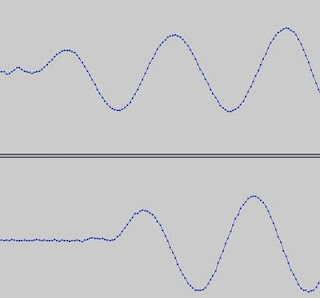
\includegraphics[width=250px]{img/100kHz_grynas.png}
  \caption{100 kHz grynojo tono gauto manekeno galvoje oscilograma (viršuje – kairioji ausis, apačioje – dešinioji}
  \label{fig:100kHz_grynas}
\end{figure}

\ref{fig:100kHz_grynas} pav. matomi grafikai atvaizduoja manekeno galvoje esančių mikrofonų parodymus esant garso šaltinio skleidžiamam garsui, kurio dažnis siekė 1000 kHz ir atstumas iki jo – apie 1,75 m. Viršutinėje \ref{fig:100kHz_grynas} pav. dalyje – kairiosios ausies mikrofono parodymai, apatinėje dalyje – dešiniosios. Iš \ref{fig:100kHz_grynas} paveikslo matome, jog tarp abiejų mikrofonų parodymų susidaro fazių skirtumas, taip pat apatinėje paveikslėlio dalyje matomas atsiradęs vėlavimas lyginant su kairiosios ausies mikrofono grafiku. Pilno signalo tarpausinis laiko skirtumas siekė 0,735 ms, ir tai yra didžiausias pasiekiamas laiko skirtumas, nes manekeno galvos priekinė dalis buvo statmena garso signalo šaltiniui.

\begin{figure}[!ht]
  \centering
  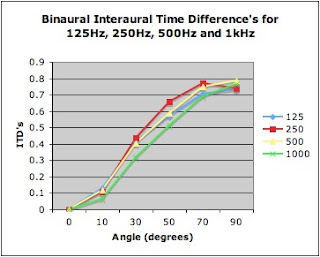
\includegraphics[width=250px]{img/TLS_degree.png}
  \caption{Tarpausinio laiko skirtumo priklausomybė nuo garso kritimo kampo.}
  \label{fig:TLS_degree}
\end{figure}

0,735 ms laiko skirtumas gali būti per didelis tarpausiniam laiko skirtumui, nes „maksimalus tarpausinis laiko skirtumas gali siekti tik 0,66 ms standartiniam žmogaus galvos dydžiui“. Taip teigiama 5-tame „Computational Auditory Scene Analysis“ knygos (išleista 2005 m) skyriuje pavadinimu „Binauralinio garso lokalizacija“. Knygos autoriai - DeLiang Wang ir Guy J. Brown. Kiti šaltiniai teigia, jog 90$^\circ$ kampo garso šaltinio padėtis prieš manekeno galvą gali sukurti 0,7 ms tarpausinį laiko skirtumą. Pastarasis straipsnis – „Binauralinė klausa“ autoriaus dr. Ruth Y. Litovsky parašytas 2008 m. Šis straipsnis parodo, jog skirtumai tarp vidutinių žmogaus galvų dydžių sudaro maksimalaus tarpausinio laiko skirtumo vertės netikrumus. Jei ši vertė tampa per didelė, tai reiškia, kad mikrofonus reikia įdėti giliau į manekeno galvą, taip norint sumažinti atstumą tarp abiejų mikrofonų.

\begin{figure}[!h]
  \centering
  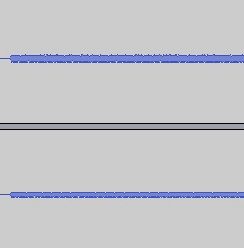
\includegraphics[width=150px]{img/125kHz_TGLS.png}
  \caption{Tarpausinis garso lygio skirtumas esant 125 kHz dažniui, kai garso šaltinio kampas manekeno galvos atžvilgiu siekia 90$^\circ$}
  \label{fig:125kHz_TGLS}
\end{figure}

\begin{figure}[!h]
  \centering
  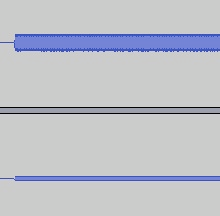
\includegraphics[width=150px]{img/1000kHz_TGLS.png}
  \caption{Tarpausinis garso lygio skirtumas esant 1 MHz dažniui, kai garso šaltinio kampas manekeno galvos atžvilgiu siekia 90$^\circ$}
  \label{fig:1000kHz_TGLS}
\end{figure}

Iš \ref{fig:125kHz_TGLS} ir \ref{fig:1000kHz_TGLS} pav. matome, jog lyginant du skirtingo dažnio garsus (125 kHz ir 1000 kHz), kai garso bangos kritimo kampas siekia 90$^\circ$, susidaro tarpausinio garso lygių skirtumas. Kaip ir buvo minėta, esant aukštesniems dažniams nei 1,5 kHz, tarpausinis laiko skirtumas tampa labai mažas ir tuomet dominuoja tarpausinis garso lygių skirtumas. Fizikinis šio fenomeno paaiškinimas būtų toks, kad esant aukštesniems dažniams, garso bangos sutankėja ir jų galimybė persilenkti aplink galvą stipriai sumažėja. Esant skirtingiems objektų dydžiams ir skirtingiems garso bangų dažniams išlieka difrakcinė priklausomybė, bet šiuo atveju tai negalioja, nes naudojama standartinė vidutinio žmogaus galvos dydžio manekeno galva. Be abejo išlieka minimalūs skirtumai, nes kiekvieno žmogaus galva turi savo unikalią formą ir dydį, o tai sukuria skirtingą šešėlinį dažnį, bet galima sakyti, jog šis skirtumas yra nykstamai mažas.

\begin{figure}[!h]
  \centering
  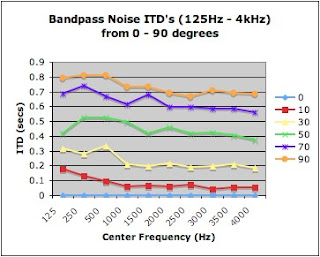
\includegraphics[width=150px]{img/ITD_freq.png}
  \caption{Tarpausinio laiko skirtumo priklausomybė dažnio esant skirtingiems garso bangos kritimo kampams (0$^\circ$ - 90$^\circ$)}
  \label{fig:ITD_freq}
\end{figure}


\subsection{Kambario impulsinis atsakas}

Kambario Impulsinis Atsakas (sutrumpintai \textit{KIA}, angl. \textit{RIR – Room Impulse Response}) – tai yra laiko domeno signalas parodantis dažnių pasiskirstymą ir amplitudės mažėjimą. Naudojant KIA daroma prielaida jog kambario erdvė yra stabili ir linijinė, laikui bėgant nekintanti sistema.

KIA inkapsuliuoja sekančius parametrus:
\begin{enumerate}
\item Garso signalo vėlinimą (angl. \textit{propagation delay}) – atstumas laike kurį garsas nukeliauja nuo garso šaltinio iki klausytojo.
\item Tiesioginį garsą (angl. \textit{direct sound}) – tiesioginis garsas atitinką maksimumą kuris nusako trumpiausią atstumą nuo garso šaltinio iki klausytojo.
\item Ankstyvuosius atspindžius (angl. \textit{early reflections}) – pirmos eilės (dažniausiai atspindį nuo grindų arba lubų), antrosios ir kitų eilių atspindžius.\item Aido liekamąją dalį (angl. \textit{reverberation tail}) – tai stochastinė aido dalis kurioje yra didelis atspindžių kiekis kurie nebegali būti suskirstyti į ankstyvuosius atspindžius.  
\item Pradinio Vėlinimo Atotrūkis (PVA, angl. \textit{ITDG – Initial Time Delay Gap}) – tai laikas tarp į klausytojo klausos sistemą atvykusio tiesioginio garso ir pirmojo ankstyvojo atspindžio (dažniausiai atsispindėjusio ne nuo grindų). Dažnai norint išvengti papildomų skaičiavimų paprastas signalo vėlinimas yra panaudojamas PVA imituoti.
\end{enumerate}

Šiame darbe yra panaudotas supaprastintas KIA modelis, darant prielaidą jog garso bangą sudaro baigtinis skaičius spindulių sklindančių tiesia linija visomis kryptimis. Ši prielaida yra klaidinga tačiau tokiu būdu yra ženkliai sumažinamas skaičiavimų kiekis kas savo ruožtu leidžia taikyti KIA modelį realiuoju laiku veikiančiame įrenginyje neturinčiame ypač didelių skaičiavimo galimybių. Priešingu atveju nepriėmus anksčiau minėtos prielaidos KIA generavimas tampa labai sudėtingas ir negali būti taikomas realaus laiko binauralinio garso generavimui.


\subsection{Skyriaus apibendrinimas}

Šiame skyriuje buvo paminėti pagrindiniai metodai susiję su binauraliniu garsu. Minimaliam binauraliniam efektui gauti pakanka tik \textit{HRTF} filtrų, bet kaip patvirtina atlikti bandymai - šis efektas nėra labai įtikinantis ir natūralus. Tačiau jei prieš panaudojant \textit{HRTF} funkcijas garso signale yra užkoduojama kambario akustinė informacija, binauralinio garso efektas tampa panašesnis į realiame pasaulyje susidarančius garsus. 
Darbo metu sukurta garso apdorojimo sistema išnaudoja šiame skyriuje aprašytus metodus sukuriant pakankamai įtikinantį binauralinį efektą.

\section{Sistemos kūrimas}

Šiame skyriuje bus aptartas sistemos kūrimas, bendra struktūros apžvalga bei aprašyti naudojami algoritmai. Pagrindinis dėmesys bus skirtas galvos orientacijos įrenginio daviklių duomenų suliejimo algoritmų bei garso binauralinio garso generavimo metodų aprašymui.

\subsection{Sistemos struktūrinė schema}

\begin{figure}[!h]
  \centering
  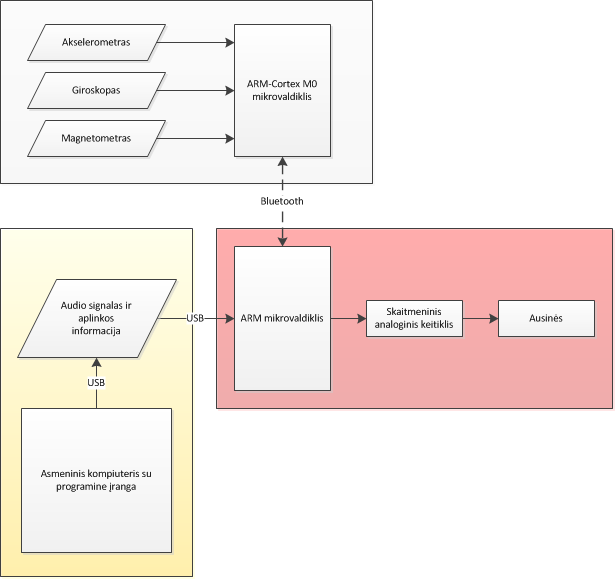
\includegraphics[width=300px]{img/schema.png}
  \caption{Struktūrinė schema}
  \label{fig:full_schematic}
\end{figure}

\ref{fig:full_schematic} pav. pavaizduota baigiamojo bakalaurinio darbo struktūrinė schema. Sistemą sudaro trys dalys:

\begin{itemize}
\item Galvos sekimo įrenginys
\item Garso apdorojimo įrenginys
\item Asmeninis kompiuteris su specializuota programine įranga.
\end{itemize}

Galvos sekimo įrenginys skirtas sekti vartotojo galvos orientacijai erdvėje, tam kad, sistemai suteikti generuojamo garso priklausomybę nuo galvos orientacijos. Ši priklausomybė yra būtina norint kuo tiksliau sugeneruoti binauralinį garsą. Norint įgyvendinti nepriekaištingą galvos sekimo įrenginio veikimą, buvo suprojektuota ir pagaminta spausdintinė plokštė, atitinkanti fizinių išmatavimų ir elektros energijos sąnaudų reikalavimus. Taip pat parašytos dvi programinės įrangos – pačiam galvos orientacijos sekimo įrenginiui bei asmeniniam kompiuteriui. Įrenginio programinė įranga skirta nuskaityti parodymus iš skirtingų jutiklių – akselerometro, magnetometro ir giroskopo, o taipogi juos siųsti į asmeninį kompiuterį tolimesniam apdorojimui. Savo ruoštu, asmeninis kompiuteris su savo programine įranga šiuos duomenis toliau apdoroja. Šiuo atveju atliekama visų daviklių duomenų filtracija ir sujungimas. Tokiu būdu išgaunama galvos orientacija trimatėje erdvėje.
Garso apdorojimo įrenginys – tai baigiamojo bakalaurinio darbo metu sukurta įterptinė sistema skirta binauralinio garso generavimui, joje apdorojami virtualios erdvės akustiniai ypatumai, o taip pat iš asmeninio kompiuterio gautas monofoninis garsas priklausomai nuo galvos sekimo įrenginio surinktų duomenų atitinkamai pakeičiamas. Šių veiksmų visuma sukuria binauralinį efektą. Tad kaip yra matoma iš paveikslo 4.1 pagrindinė sistemos dalis yra garso apdorojimo įrenginys, tačiau neturint tiek virtualios, tiek realios aplinkos duomenų tikrą binauralinį efektą sukurti neįmanoma. Garso apdorojimo įrenginys susideda iš kelių dalių – galingas 32 bitų ARM serijos mikrovaldiklis su integruotu skaitmeninių signalų apdorojimo moduliu, maitinimo stabilizatoriaus, sąsajų bei skaitmeninio – analoginio keitiklio. Pastarasis skirtas skaitmeninį apdorotą signalą paversti į analoginį garso toną. 

\subsection{Jutiklių duomenų sintezės filtras}

Sensor fusion algoritmas yra naudojamas galvos orientacijos nuskaitymo įrenginyje. Galvos orientaciją erdvėje nuskaito trys davikliai: 

triašis akselerometras – pagreičiui kiekvienoje ašyje nustatyti.
\begin{itemize}
\item triašis magnetometras – nustatyti kampą žemės magnetinių linijų ir magnetometro atžvilgiu.
\item Triašis giroskopas – kampiniam pagreičiui trijose ašyse nustatyti.
\end{itemize}

Visi šie trys davikliai turi savo stipriąsias ir silpnąsias puses, tačiau sensor fusion algoritmai padeda padidinti galutinių duomenų tikslumą. Dažniausiai naudojamas filtras – Kalmano, tačiau dėl didelio matematinio skaičiavimo kiekio (kuris neigiamai įtakoja bendrą mažos galios įterptinės sistemos greitaveiką) šiame darbe buvo pasirinktas paprastesnis Madgwick sensof fusion filtras. Palyginus su Kalmano filtru, Madgwicko filtras turi tik vieną žingsnį per kurį yra apskaičiuojami galutiniai duomenis, atsisakius nuspėjimo ir korekcijos žingsnių (kurie naudojami Kalmano filtre) sutaupomas laikas, ko pasekoje padidėja greitaveika. Tačiau atsisakius prieš tai minėtų dviejų žingsnių suprastėja filtro savybės, nes neatsižvelgiama į prieš tai buvusius duomenis.


\end{document}